\documentclass[
	openany,
	% -- opções da classe memoir --
	12pt,% tamanho da fonte
   % openright,
	%twoside,
    oneside,
    % para impressão em verso e anverso. Oposto a oneside
	a4paper,			% tamanho do papel. 
	brazil				% o último idioma é o principal do documento
	]{abntex2}

% ---
% Pacotes básicos 
% ---

\usepackage{fontspec}
\setmainfont{Arial}

\usepackage[utf8]{inputenc}		% Codificacao do documento (conversão automática dos acentos)
\usepackage{indentfirst}		% Indenta o primeiro parágrafo de cada seção.
\usepackage{color}				% Controle das cores
\usepackage{graphicx}			% Inclusão de gráficos
\usepackage{microtype} 			% para melhorias de justificação
\usepackage{multicol}			% multiplas colunas no texto
\usepackage{subcaption}
\usepackage{caption}
\usepackage{float}
\usepackage{amsmath}
\usepackage{amssymb}
\usepackage{amsthm}
\usepackage{lipsum}
\usepackage{blindtext}
\usepackage{url}
\usepackage{listings}


% ---
% ---
% Pacotes de citações
% ---
\usepackage[brazilian]{backref}	 % Paginas com as citações na bibl
\usepackage[alf]{abntex2cite}	% Citações padrão ABNT

% --- 
% CONFIGURAÇÕES DE PACOTES
% --- 

% ---
% Configurações do pacote backref
% Usado sem a opção hyperpageref de backref
\renewcommand{\backrefpagesname}{Citado na(s) página(s):~}
% Texto padrão antes do número das páginas
\renewcommand{\backref}{}
% Define os textos da citação
\renewcommand*{\backrefalt}[4]{
	\ifcase #1 %
		Nenhuma citação no texto.%
	\or
		Citado na página #2.%
	\else
		Citado #1 vezes nas páginas #2.%
	\fi}%
% ---

% ---
% Informações de dados para CAPA e FOLHA DE ROSTO
% ---
\titulo{Comparação entre protocolos de comunicação na camada de aplicação para IoT}
\autor{Raphael Felipe Ramos Duarte Soares}
\local{Recife}
\data{2019}
\orientador{Glauco Estácio Gonçalves}
\coorientador{Victor Wanderley Costa de Medeiros}


\instituicao{%
	Universidade Federal Rural de Pernambuco -- UFRPE
  	\par
  	Departamento de Estatística e Informática
    \par
  	Curso de Bacharelado em Sistemas de Informação
}

\tipotrabalho{Trabalho de Conclusão de Curso}
% O preambulo deve conter o tipo do trabalho, o objetivo, 
% o nome da instituição e a área de concentração 
\preambulo{Monografia apresentada ao Curso de Bacharelado em Sistemas de Informação da Universidade Federal Rural de Pernambuco, como requisito parcial para obtenção do título de Bacharel em Sistemas de Informação.}
% ---


% ---
% Configurações de aparência do PDF final

% alterando o aspecto da cor azul
\definecolor{blue}{RGB}{41,5,195}
% alterando a cor de fundo dos blocos de código
\definecolor{codeBackground}{RGB}{248,248,250}

% definindo o estilo dos blocos de código
\lstset{ 
  backgroundcolor=\color{codeBackground}   % choose the background color;
}
\lstdefinestyle{code}{
    tabsize=4,
    numberstyle={\tiny},
    numbers=left,
}

% informações do PDF
\makeatletter
\hypersetup{
     	%pagebackref=true,
		pdftitle={\@title}, 
		pdfauthor={\@author},
    	pdfsubject={\imprimirpreambulo},
	    pdfcreator={LaTeX with abnTeX2},
		colorlinks=true,       		% false: boxed links; true: colored links
    	linkcolor=blue,          	% color of internal links
    	citecolor=blue,        		% color of links to bibliography
    	filecolor=magenta,      		% color of file links
		urlcolor=blue,
		bookmarksdepth=4
}
\makeatother
% --- 

% --- 
% Espaçamentos entre linhas e parágrafos 
% --- 

% O tamanho do parágrafo é dado por:
\setlength{\parindent}{1.3cm}

% Controle do espaçamento entre um parágrafo e outro:
\setlength{\parskip}{0.2cm}  % tente também \onelineskip

% ---
% compila o indice
% ---
\makeindex
% ---

% ----
% Início do documento
% ----
\begin{document}

% Seleciona o idioma do documento (conforme pacotes do babel)
%\selectlanguage{english}
\selectlanguage{brazil}

% Retira espaço extra obsoleto entre as frases.
\frenchspacing 

% ----------------------------------------------------------
% ELEMENTOS PRÉ-TEXTUAIS
% ----------------------------------------------------------
% \pretextual
%\begin{figure}[h]
%\centering % este comando é usado para centralizar a figura
%
\includegraphics[width=7cm]{figuras/logo_ufrpe_horizontal.png}\\
%\end{figure}

% \begin{figure}[ht]
% \centering
% \begin{minipage}[b]{0.45\textwidth}
% 
\includegraphics[height=3cm]{figuras/logo_ufrpe_horizontal.png}
% \end{minipage}
% \qquad
% \begin{minipage}[b]{0.45\textwidth}
% 
\includegraphics[height=2.5cm]{figuras/logo_bsi.pdf}
% \end{minipage}
% \end{figure}

%\begin{minipage}[t]{1\textwidth}
	\begin{figure}[ht]
		
\includegraphics[height=3cm]{figuras/logo_ufrpe_horizontal.png}
		\hspace{4.5cm}
    	
\includegraphics[height=2.5cm]{figuras/logo_bsi.pdf}
	\end{figure}    
%\end{minipage}

% ---
% Capa
% ---
\imprimircapa
% ---
% ---
% Folha de rosto
% (o * indica que haverá a ficha bibliográfica)
% ---
\imprimirfolhaderosto
% ---

% dedicatoria
\begin{dedicatoria}
	\vspace*{\fill}
	\centering
	\noindent
	\textit{À \ldots\\} \vspace*{\fill}
\end{dedicatoria}

% agradecimentos
\begin{agradecimentos}
Agradeço à \ldots

\end{agradecimentos}

% epigrafe
\begin{epigrafe}
    \vspace*{\fill}
	\begin{flushright}
    	\textit{``...E no final tudo se resume a 1s e 0s.''}
% 		\textit{``...E no final tudo se resume a 1s e 0s.'' \\
% 		(Charles Chaplin)}
	\end{flushright}
\end{epigrafe}

% resumo e abstract
\setlength{\absparsep}{18pt} % ajusta o espaçamento dos parágrafos do resumo
\begin{resumo}
 
No primeiro semestre de 2018 chegamos a marca de 17 bilhões de dispositivos conectados à Internet em todo o mundo. Desses 17, 10 bilhões são equipamentos como smartphones, tablets e notebooks, e 7 bilhões são os chamados IoT (Internet of Things, ou Internet das Coisas), ou seja, são "coisas" que estão conectadas à rede, mas que essa conexão não está entre suas principais funções. Isso implica dizer que hoje, há um número gigantesco de máquinas conversando com maquinas...

Baseado nisto, o presente trabalho propõe avaliar os 6 protocolos de comunicação mais comuns, HTTP, MQTT, CoAP, AMQP, STOMP e XMPP, utilizados na camada de aplicação para o envio de dados entre dispositivos, e elencar os mais rápidos, robustos e confiáveis. Para tal, foi elaborado um experimento utilizando uma placa Raspberry Pi, servindo como dispositivo IoT, um notebook e um switch. O experimento consistiu no envio, utilizando os protocolos mencionados anteriormente, de uma certa quantidade de dados reais, extraídos de uma estação meteorológica, partindo da placa Rasp para o notebook. Para deixar o experimento o mais próximo possível da realidade, foi utilizado um simulador de redes para emular uma rede de baixa qualidade. Os pacotes de dados enviados foram capturados e foi realizada uma análise estatística para comparar 3 fatores: velocidade, latência e perda de pacotes. A partir do resultado dessa análise foi possível elencar os melhores protocolos e uma sugestão dos seus possíveis usos.

 \textbf{Palavras-chave}: Internet das Coisas, Protocolos, Camada de Aplicação, Raspberry Pi, HTTP, MQTT, CoAP, AMQP, STOMP, XMPP.
\end{resumo}


\begin{resumo}[Abstract]
 	\begin{otherlanguage*}{english}
  
  		\lipsum[1] 

   		\vspace{\onelineskip}
 
		\noindent 
		\textbf{Keywords}:  word 1, word 2, \ldots.
 	\end{otherlanguage*}
\end{resumo}

% ---
% inserir lista de ilustrações
% ---
\pdfbookmark[0]{\listfigurename}{lof}
\listoffigures
\cleardoublepage
% ---

% ---
% inserir lista de tabelas
% ---
\pdfbookmark[0]{\listtablename}{lot}
\listoftables*
\cleardoublepage
% ---

% ---
% inserir lista de abreviaturas e siglas
% ---
\begin{siglas}
	\item[IoT] Internet of Things (Internet das Coisas)
	\item[API] Application programming interface
	\item [RTT] Round Trip Time
	\item[HTTP] Hypertext Transfer Protocol	
	\item[OSI] Open System Interconnection
	\item[UDP] User Datagram Protocol	
	\item[TCP] Transmission Control Protocol
	\item[IP] Internet Protocol
	\item[MQTT] Message Queuing Telemetry Transport
	\item [CoAP] Constrained Application Protocol
	\item [DDS] Data Distribution Service
	\item [AMQP] Advanced Message Queuing Protocol
	\item [STOMP] Simple (or Streaming) Text Orientated Messaging Protocol
	\item [XMPP] Extensible Messaging and Presence Protocol
\end{siglas}
% ---

% ---
% inserir o sumario
% ---
\pdfbookmark[0]{\contentsname}{toc}
\tableofcontents*
\cleardoublepage
% ---



% ----------------------------------------------------------
% ELEMENTOS TEXTUAIS
% ----------------------------------------------------------
\textual

% ----------------------------------------------------------
% inclusao das secoes do texto
% ----------------------------------------------------------
\chapter{Introdução}

\section{Apresentação}

No primeiro semestre de 2018 a humanidade alcançou a marca de 17 bilhões de dispositivos conectados \cite{url_lueth2018_7BiIoT}. O avanço tecnológico e a computação ubíqua chegaram a tal ponto que hoje a expressão "navegar na internet" ou "surfar na rede" está defasada, "mergulhar na rede" talvez seja o termo mais apropriado. A sociedade moderna está tão cercada por e imersa na tecnologia no seu cotidiano que chega a ser difícil encontrar, no ambiente urbano, uma pessoa sem acesso à Internet.

Dentre estes 17 bilhões há um nicho de 7 bilhões que vem crescendo de forma quase exponencial nos últimos anos e com perspectiva de crescer muito mais, são os dispositivos de Internet das Coisas (Internet of Things, ou IoT). Dispositivos IoT são basicamente objetos que possuem alguma tecnologia embarcada, sensores e conexão com Internet, tornando-os capazes de coletar, transmitir e, em alguns casos, processar dados \cite{artigo_santos2016_IoTDaTeoriaAPratica}. Hoje já existe uma enorme variedade deles no mercado, tais como lâmpadas, geladeiras, micro-ondas inteligentes, e outros tantos chamados "dispositivos inteligentes". A expectativa é que eles estejam cada vez mais inseridos no cotidiano das pessoas, pois é esperado um crescimento de 10 bilhões de dispositivos IoT em 2020 e 22 bilhões em 2025. Em paralelo a esta expansão, há uma prospecção de crescimento do mercado global de IoT de 37\% em 2018, saltando de U\$ 110 bilhões para U\$ 151 bilhões e com perspectiva de chegar a U\$ 1,56 trilhão em 2025 \cite{url_lueth2018_7BiIoT}.

Atualmente já existem diversos exemplos de como estes dispositivos podem ajudar a sociedade em suas atividades diárias, tanto no individual quanto no coletivo. Na medicina, no monitoramento dos sinais vitais e condições de saúde dos pacientes em hospitais e em casas de idosos. Nas residências, nas medições de consumo de energia remotamente e monitoramento de câmeras de segurança à distância. No transporte, com sensores de proximidade nos carros ajudando a evitar colisões e controle de tráfego nas vias ajudando a melhorar o trânsito. Na agricultura, com sensores de temperatura, umidade e luminosidade nas fazendas e plantações ajudando a otimizar a produção de comida \cite{artigo_mancini2017_iotAplicacoes}.

Apesar do progresso científico estar avançando consideravelmente neste setor, por ser um campo relativamente recente, a tecnologia para realizar de forma satisfatória e eficaz a comunicação entre estes objetos, também chamada comunicação Maquina-para-Maquina (em inglês: Machine to Machine, ou M2M) ainda é muito incipiente. É bastante comum haver falha no envio de informações entre estes dispositivos, seja por problemas de conectividade ou de rede, seja por quebra ou desligamento inesperado de um equipamento, seja por manutenção incorreta ou escassa, ou por algum outro fator externo [PROCURAR UMA REFERENCIA!!!]. O fato é que a troca de informações entre dispositivos IoT é um fator crucial para o avanço e solidificação dessa tecnologia e precisa ser estudado com mais atenção. 

Com base nisto, este trabalho se propõe a analisar e comparar 6 protocolos de comunicação mais comumente utilizados em dispositivos IoT para transferência de dados na camada de aplicação. São eles: HTTP, MQTT, CoAP, XMPP, AMQP e STOMP. Para tal foi realizado um experimento seguindo os moldes de design de experimentos em que foi utilizada uma placa Raspberry Pi como dispositivo IoT cuja responsabilidade foi o envio de dados, utilizando cada um dos 6 protocolos mencionados, capturados previamente de uma estação meteorológica, e um notebook como servidor de aplicação que foi responsável pelo recebimento destes dados enviados. Os pacotes de dados transferidos da placa para o notebook foram capturados, tratados analisados e comparados. Através desta comparação foi possível chegar ao objetivo do trabalho.


\section{Motivação e Justificativa}

Como mencionado anteriormente, a área de Internet das Coisas vem num crescimento constante e, a medida que os avanços tecnológicos vão progredindo, os custos de produção desses dispositivos vão barateando e se popularizando cada vez mais.  

Apesar desses avanços, a comparação entre protocolos M2M não foi alvo de muitos estudos e, dentre estes, a extensa maioria deles se focou nos 2 mais utilizados, o MQTT e o CoAP.

Além de concentrar uma boa quantidade de protocolos de comunicação IoT, cujas arquiteturas diferem bastante entre si, este estudo inclui também, como um dos protocolos de comparação, o HTTP, que é o protocolo mais tradicional e amplamente utilizado hoje em dia na Internet.


\section{Objetivos}

O presente trabalho tem por objetivo principal avaliar e comparar a eficiência dos protocolos de comunicação nos dispositivos de Internet das Coisas. Através desta comparação pretende-se atender os seguintes objetivos específicos:

\begin{itemize}
    \item Avaliar os protocolos quanto ao atraso no tempo de envio e de recebimento dos pacotes;
    \item Avaliar os protocolos quanto a quantidade de dados trafegada por segundo;
    \item Avaliar os protocolos no quesito de quantidade de pacotes extras gerados durante a comunicação;
    \item Avaliar os protocolos quanto a quantidade e porcentagem de pacotes perdidos com relação a quantidade total de pacotes enviados;
\end{itemize}


\section{Organização do Trabalho}

O presente trabalho está organizado em seis capítulos. O capítulo atual que visa introduzir o contexto geral em que problema se encontra inserido, além da motivação, justificativa e objetivos que nortearam sua execução. O demais capítulos se encontram divididos da seguinte maneira:

\textbf{Capítulo 2}: Trata da fundamentação teórica, onde são apresentados os conceitos envolvidos no trabalho, bem como a arquitetura e o \textit{modus operandi} de cada protocolo.

\textbf{Capítulo 3}: São discutidos alguns trabalhos relacionados cujo objeto de estudo também é a comparação entre protocolos de comunicação.

\textbf{Capítulo 4}: Apresenta a metodologia e arquitetura empregada no experimento, juntamente com os métodos de captura dos dados para análise.

\textbf{Capítulo 5}: Expõe e discute os resultado a partir análise e interpretação dos dados obtidos.

\textbf{Capítulo 6}: Traz as considerações finais do trabalho, junto com suas contribuições, objetivos alcançados e dificuldades encontradas, e propõe possíveis trabalhos futuros.
\chapter{Fundamentação teórica}

\section{Considerações iniciais}
Neste capítulo introduzimos os conceitos que serão abordados durante o desenvolvimento deste trabalho. A seção~\ref{sec:arquiteturas} traz uma explanação sobre as arquiteturas que os protocolos abordados neste trabalho fazem uso. A Seção~\ref{sec:protocolos} apresenta uma visão geral sobre cada um dos protocolos utilizados bem como seu funcionamento e características.

\section{Arquiteturas}
\label{sec:arquiteturas}

De modo geral existem dois principais padrões para transmissão de mensagens na camada de aplicação entre computadores conectados em rede, são eles: requisição-resposta (do inglês, request-response) e publicação-assinatura (do inglês, publish-subscribe).

\subsection{Requisição-Resposta}

O padrão requisição-resposta funciona da seguinte forma, um computador envia uma requisição de algum dado através de um canal, nesse caso a rede, e um outro computador recebe essa requisição, processa esse recebimento e envia uma resposta de volta \cite{livro_hohpe2003_enterpriseIntegrationPattern}. Esse procedimento é análogo a uma ligação telefônica, em que uma pessoa, requisitante, liga solicitando alguma informação através de um canal, nesse caso a rede de telefonia, e outra pessoa responde, atendendo essa solicitação.

Esse padrão é extremamente comum na Internet hoje, pois é o padrão utilizados pelos navegadores. Quando uma pessoa digita uma URL num navegador, este faz uma requisição utilizando o protocolo HTTP, que será detalhado mais adiante, a um servidor e este por sua vez, ao receber a requisição, processa e geralmente devolve como resposta um texto no formato HTML que é interpretado pelo navegador e utilizado para renderizar a página em questão \cite{url_mozilla2018_httpOverview}

Na extensa maioria dos casos este padrão é implementados de forma síncrona, ou seja, ao realizar uma requisição, o requisitante permanece esperando até obter uma resposta do destinatário ou até o período máximo de espera (timeout) ser atingido. Entretanto, em alguns casos, este padrão pode ser implementado de forma assíncrona, ou seja, não há necessidade de espera por parte do solicitante após a realização da requisição. Neste caso cabe ao destinatário da solicitação entrar em contato com o requerente para devolver-lhe o resultado do seu requerimento FONTE: \url{ https://www.w3.org/Protocols/HTTP/1.1/rfc2616bis/draft-lafon-rfc2616bis-03.html#rfc.section.1}. Um exemplo de requisição assíncrona é o envio de email, onde não é necessário que o remetente permaneça esperando uma resposta do destinatário.

\subsection{Publicação-Assinatura}

No padrão publicação-assinatura, ao contrário do padrão requisição-resposta, a troca de mensagens entre o remetente e o destinatário não ocorre de forma direta. Neste padrão existem 3 agentes, o publicador, o assinante e a central. 

A comunicação entre os agentes ocorre da seguinte forma: o publicador envia sua mensagem para a central contendo o conteúdo da mensagem e o tópico ou categoria da mensagem. O assinante, por sua vez, envia para a central uma solicitação de assinatura para um determinado tópico ou categoria. É permitido ao assinante possuir quantas assinaturas quiser. A central funciona como um intermediário e é responsável por receber mensagens de publicadores e por aceitar e registrar solicitações de assinaturas. Ao receber uma mensagem de um publicador, a central verifica quantos e quais são os assinantes do tópico daquela mensagem e então os envia a referida mensagem. 

As duas principais vantagens desse padrão são a independência e a escalabilidade. Independência pois não existe nenhuma correlação entre publicadores e assinantes, eles não precisam ter conhecimento da existência um do outro, inclusive é factível a presença de publicadores de um determinado tópico sem que hajam assinantes e vice-versa. A escalabilidade refere-se a potencial de crescimento da rede através da inclusão nós, seja elem publicador ou assinante, neste tipo de rede. Não se faz necessário alterações na topologia da rede para adição ou remoção de um nó, pois o padrão já dá suporte a este tipo de operação.

\section{Protocolos}
\label{sec:protocolos}
Neste trabalho vamos utilizar um total de 6 protocolos mais difundidos para comunicação M2M (Machine-to-Machine). São eles:
\begin{enumerate}
\item HTTP
\item CoAP
\item MQTT
\item AMQP
\item STOMP
\item XMPP
\end{enumerate}

\subsection{HTTP}

\subsubsection*{O que é ?}
O Hypertext Transfer Protocol (HTTP), ou Protocolo de Transferência Hipertexto em português, é um protocolo de comunicação, localizado na camada de aplicação (a última camada no modelo OSI). Ele é utilizado em sistemas de informação com o objetivo de transmitir documentos em hipermídia, distribuídos e colaborativos. Hipermídia é a reunião de vários tipos de mídias, tais como imagens, vídeos, sons e texto, em um documento no ambiente computacional, que são navegáveis, interativos e cuja leitura se dá de forma não linear. Qualquer página na Web é um ótimo exemplo de um documento de hipermídia. 

O desenvolvimento do HTTP é coordenado pela World Wide Web Consortium (W3C) e pela Internet Engineering Task Force (IETF) e tem sido a principal forma de comunicação na World Wide Web desde que foi criado, em 1990. Na sua primeira versão HTTP/0.9, seu único objetivo era a transferência simples de dados através da internet. Na sua segunda versão, a 1.0, o procotolo foi melhorado, foi incluído os headers, que continham informações sobre o que estava sendo trafegado. Também foi incluído nesta versão o modelo request-response, ou requisição-resposta, para informar se a comunicação foi realizada com sucesso ou não. Atualmente o HTTP está na versão 2.0 e diversas melhorias foram acrescidas, como compressão de headers, definição de prioridade nas requisições, entre outas.

\subsubsection*{Características}
Com relação as características do HTTP, pode-se dizer que ele é:
\begin{itemize}
\item Simples: as mensagens em HTTP foram desenhadas para serem fáceis de ler e entender por humanos sem necessitar de nenhum tipo de aparato extra;
\item Extensível: os cabeçalhos das mensagens HTTP foram criados de forma a propiciar a adição de novas propriedades de maneira fácil e intuitíva;
\item Stateless: o protocolo foi criado para não manter estado, ou seja, cada requisição é totalmente independente uma da outra. Não há compartilhamento de dados entre duas requisições diferentes.
\item Confiabilidade: Como HTTP envia seus dados através da camada de transporte TCP/IP, ele é um protocolo considerado seguro, pois os dados trafegados não se perdem "silenciosamente". 
\end{itemize}


\subsubsection*{Como funciona ?}
O HTTP funciona no modelo request-response utilizando uma arquitetura cliente-servidor. Quando nós abrimos um Web Browser, como Google Chrome, Mozilla Firefox ou Internet Explorer e digitamos uma URL, esse navegador é o cliente da nossa arquitetura e ele está fazendo uma requisição HTTP a uma aplicação hospedada em um computador em outra parte do globo, que é o servidor. Esse servidor, por sua vez, ao receber essa requisição, realiza o processamento desta e retorna uma resposta ao cliente. Essa resposta contém informações sobre este processamento e pode ou não conter o conteúdo solicitado no corpo da mensagem.

As mensagens trocadas entre o cliente e o servidor http possuem uma estrutura predefinida. Essa estrutura é constituída por 3 partes, a Request-Line, ou linha inicial, o Header, ou cabeçalho, e o Body, ou corpo da mensagem. 
A Request-line é a primeira linha da requisição. Caso esta seja uma solicitação enviada pelo cliente, nós temos o tipo de método da solicitação e a versão do protocolo que estamos utilizando. Caso seja uma resposta do servidor, nós temos a versão do protocolo seguido pelo código da resposta da mensagem. Os códigos mais comuns são: 200 - indica que a solicitação foi processada com sucesso, 400 - indica que a requisição está com algum erro de sintaxe, 401 - indica que está tentando acessar um recurso cuja permissão é restrita e é necessário informar alguma credencial, 403 - indica que a requisição é válida, e que o usuário foi autenticado, mas não possui permissão para acessar o recurso, 404 - indica que o recurso que está sendo solicitado não foi encontrado. 
Da segunda linha em diante vem o Header, que contém uma série de informações sobre a requisição em si, tais como data/hora, endereço e tipo do servidor, tamanho e tipo do conteúdo de retorno da resposta, entre outros.
Após o término do Header, vem uma linha em branco e em seguida vem o body, que é opcional, com o conteúdo da mensagem em si. Quando acessamos uma URL, é no body que o servidor manda o arquivo html que é renderizado na tela do browser.

O HTTP utiliza uma série de métodos para indicar qual é a ação desejada pelo cliente ao servidor. São ao todo 9 métodos, mas 4 são os mais utilizados, são eles: GET, POST, PUT e DELETE. Cada um deles possui uma semântica própria, mas eles compartilham algumas características em comum. Abaixo segue uma breve descrição do que cada método faz.
\begin{itemize}
\item GET: é um método responsável por buscar informações. Esse método pode ou não ter conteúdo no corpo da resposta;
\item HEAD: é um método idêntico ao GET, porém não poussui conteúdo no corpo da resposta;
\item POST: é um método responsável por submeter informações ao servidor. Normalmente é utilizado para causar mudanças de estados no mesmo;
\item PUT: também é um método de submissão, porém é comumente utilizado para atualizar informações já presentes no servidor;
\item DELETE: é responsável por deletar recursos específicos;
\item CONNECT: é responsável por criar um túnel de conversasão entre o cliente e o servidor. Normalmente requer algum tipo de autenticação por parte do cliente;
\item OPTIONS: é usado para obter as opções de requisição permitidas para um determinado recurso no servidor;
\item TRACE: é utilizado para obter o caminho que a requisição faz até o servidor. É retornado para o cliente quais proxys e máquinas a sua requisição passa até chegar ao destino;
\item PATCH: é um método utilizado para realizar alterações parciais em um derterminado recurso;
\end{itemize}


FONTES:
\url{https://pt.wikipedia.org/wiki/Hypertext_Transfer_Protocol}
\url{https://developer.mozilla.org/en-US/docs/Web/HTTP/Overview}
\url{https://developer.mozilla.org/en-US/docs/Web/HTTP/Status}
\url{https://www.digitalocean.com/community/tutorials/how-to-troubleshoot-common-http-error-codes}
\url{https://hpbn.co/brief-history-of-http/}
\url{https://en.wikipedia.org/wiki/Hypertext_Transfer_Protocol}
\url{https://developer.mozilla.org/en-US/docs/Web/HTTP}
\url{https://developer.mozilla.org/en-US/docs/Web/HTTP/Methods}
\url{https://www.w3.org/Protocols/rfc2616/rfc2616.html}
\url{https://developer.mozilla.org/en-US/docs/Web/HTTP/Resources_and_specifications}
\url{https://www.w3.org/Protocols/Specs.html}
\url{https://www.w3.org/Protocols/HTTP/1.1/rfc2616bis/draft-lafon-rfc2616bis-03.html#rfc.section.1}
\url{https://pt.wikipedia.org/wiki/Hiperm%C3%ADdia}
\url{https://pt.wikipedia.org/wiki/Design_de_hiperm%C3%ADdia}


\subsection{CoAP}

\subsubsection*{O que é ?}
O Constrained Application Protocol (CoAP) é um protocolo para web da camada de aplicação, criado pela Internet Engineering Task Force (IETF)  especificamente para ser utilizado na comunicação entre máquinas (Machine-to-machine ou M2M) que sejam por elas mesmas limitadas, como disporem de uma fonte de energia restrita ou possuírem baixo poder de processamento ou armazenamento, ou estejam imersos em redes limitadas ou que possuam restrições de alguma forma, seja por uma alta taxa de perda de pacotes, ou por uma baixa velocidade de banda ou por qualquer outro motivo.	

\subsubsection*{Características}
Por ter sido criado no modelo REST, uma das grandes vantagens de se utilizar o CoAP é a integração facilitada com o protocolo HTTP, que é o protocolo mais utilizado na web. Outra característica importante deste protocolo é possuir um cabeçalho pequeno, limitado a 4 bytes, resultando numa diminuição do tamanho do pacote como um todo e na priorização do conteúdo da mensagem em si. Este cabeçalho é constituído de, entre outras coisas, um identificador da mensagem, um token e um tipo da mensagem. O identificador serve para o CoAP detectar mensagens em duplicidade. O Token por sua vez, permite o CoAP relacionar as mensagens de requisição com a sua resposta. O tipo de mensagem pode variar entre confirmable ou confirmável (CON), Non-confirmable ou não-confirmável (NON), acknowledgement ou recebido (ACK) e reset ou resetar (RST). Esta tupla de id, token e tipo tornam possível uma outra característica fundamental do CoAP que é o suporte a mensagens assíncronas, ou seja, o cliente pode fazer uma requisição ao servidor, e este por sua vez não responder imediatamente e sim depois de um certo tempo. Algumas outras características do CoAP incluem o suporte a descoberta, suporte multicast e suporte a content-type, do mesmo modo que o HTTP. 

\subsubsection*{Como funciona ?}
Como o CoAP foi criado baseado no modelo REST, funciona de maneira muito similar ao HTTP. Na troca de mensagens existe um servidor que disponibiliza recursos através de uma URL, e um cliente, que acessa esses recursos fazendo uma requisição a esta URL utilizando os mesmos métodos do HTTP: GET, POST, PUT e DELETE. Porém ao contrário do HTTP, o CoAP foi desenvolvido utilizando UDP na camada de transporte, e por isso necessitou implementar seus próprios métodos de detecção de duplicidade, retransmissão de pacotes e confiabilidade. Para tratar a confiabilidade o CoAP se utiliza do tipo de mensagem CON. Quando um nó (cliente ou servidor) envia uma requisição deste tipo, ele espera receber um outra requisição do tipo ACK como resposta, informando que o outro lado recebeu a requisição enviada. A figura \ref{fig:coap_success} ilustra uma requisição CoAP do tipo CON feita por um cliente utilizando o método GET solicitando o valor da temperatura. Na requisição da esquerda a temperatura é retornada com sucesso pelo servidor no conteúdo mensagem ACK. Na requisição da direita, é retornado o erro 404 informando que o recurso solicitado não foi encontrado.

\begin{figure}[h]
\centering
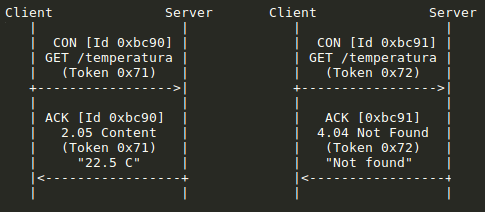
\includegraphics[height=5cm]{figuras/coap_request_success.png}
\caption{Exemplo de requisição CoAP do tipo CON e da resposta ACK}
\label{fig:coap_success}
\end{figure}

Caso o outro lado não devolva esta mensagem esperada, o nó solicitante  aguarda o tempo de timeout definido e então envia novamente a mensagem CON, e continua reenviando até receber a resposta ACK esperada. A figura \ref{fig:coap_timeout} ilustra o reenvio da requisição por parte do cliente após timeout até o recebimento da resposta ACK do servidor. Por outro lado, mensagens do tipo NON são não confirmáveis, ou seja, não necessita receber uma mensagem ACK como resposta.

\begin{figure}[h]
\centering
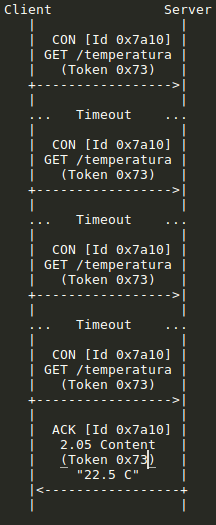
\includegraphics[height=13cm]{figuras/coap_request_timeout.png}
\caption{Exemplo de reenvio da requisição CoAP do tipo CON após o timeout}
\label{fig:coap_timeout}
\end{figure}

Como já mencionado anteriormente, o CoAP faz uso de um token no cabeçalho para possibilitar o envio de mensagens assíncronas. Este token é utilizado para relacionar as mensagens. Quando um cliente envia uma requisição para um servidor requisitando um recurso, seja ela do tipo CON ou NON, nesta requisição há um token, e o servidor, ao responder, faz uso deste mesmo token na mensagem de resposta. Caso a mensagem solicitada seja CON e o servidor não puder enviar o conteúdo da resposta imediatamente, ele envia uma mensagem ACK vazia e, após algum tempo, envia a resposta também utilizando o mesmo token inicial. A figura \ref{fig:coap_token} ilustra bem a situação mencionada acima.

\begin{figure}[h]
\centering
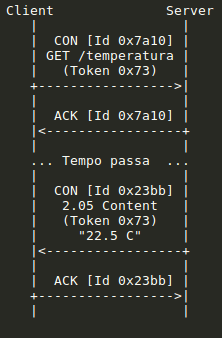
\includegraphics[height=8cm]{figuras/coap_request_token.png}
\caption{Exemplo de uso do token relacionando diferentes requisições CoAP}
\label{fig:coap_token}
\end{figure}

FONTES
http://coap.technology/
https://tools.ietf.org/html/rfc7252


\subsection{MQTT}

O Message Queuing Telemetry Transport (MQTT) é um protocolo de comunicação entre máquinas (M2M ou Machine-to-Machine) e foi desenhado em cima de certos princípios que o torna ideal para ser utilizado em aplicações para Internet das Coisas. Os princípios que o MQTT se baseia são de minimizar a quantidade de banda consumida e de recursos utilizados do dispositivo em que está rodando, tentando manter a confiabilidade e assegurar que a mensagens serão entregues com sucesso. Ele é um protocolo extremamente leve que funciona usando uma arquitetura publish-subscribe para enviar e receber mensagens. Ele é bastante eficiente quando utilizado em ambientes onde a rede é de baixa qualidade e/ou quando é necessário que as mensagens transmitidas contenham a menor quantidade possível de dados "extras", para que cada pacote de dados enviados possa ser aproveitado ao máximo.

\subsubsection*{Características}

Dentre as características do MQTT estão o fato dele utilizar os protocolos TCP/IP para transmitir suas mensagens, garantindo desse modo a não perda de pacotes durante a transmissão dos dados. Além disso ele utiliza a arquitetura publicação-assinatura, que provê para ele uma distribuição de mensagens de um para muitos, ou seja, um publica e vários recebem. Ademais o protocolo minimiza a sobrecarga durante a troca de mensagens no intento de reduzir a quantidade de dados enviados na rede. 

Outra característica importante do MQTT refere-se a qualidade do serviço durante a entrega das mensagens aos assinantes. Ele dispões de 3 tipos de serviços de entrega de mensagens: "no máximo 1", "pelo menos 1" e "exatamente 1". "No máximo 1" que dizer que a mensagem tentará ser entregue 1 vez apenas e não haverá tentativa de reenvio caso haja perda. "Pelo menos 1" quer dizer que a mensagem será entregue, porém pode haver duplicidade, ou seja, a mesma mensagem enviada mais de uma vez. "Exatamente 1" quer dizer que há garantia que a mensagem será entregue e que não haverá duplicidade.

FONTE: http://docs.oasis-open.org/mqtt/mqtt/v3.1.1/os/mqtt-v3.1.1-os.html

\subsubsection*{Como funciona}


FONTE:
\url{http://mqtt.org}


\subsection{AQMP}

\subsubsection*{O que é?}
AMQP ou Advanced Message Queuing Protocol é um padrão aberto para envio de mensagens utilizando filas criado em 2003. Ele foi criado para prover a troca de mensagens de forma eficiente entre uma gama de aplicações e padrões de comunicação diferentes. 


\subsection{STOMP}

\subsubsection*{O que é?}

STOMP deriva do acrônimo em inglês Simple Text Oriented Message Protocol, ou Protocolo Orientado a Mensagens de Texto Simples em tradução livre. Sua criação foi baseado no protocolo HTTP no que tange ao escopo das mensagens, porém a troca de mensagens utiliza o padrão publicação-assinatura. Por ter sido criado nos moldes HTTP, este protocolo também possui os mesmo agentes: um Cliente e um Servidor. Este protocolo foi criado através da necessidade de se conectar a centrais de mensagens empresariais utilizando linguagens orientadas a script como Python, Ruby e Perl, visando prover o câmbio de mensagens assíncronas da forma mais básica e simples possível \cite{url_stomp2018_stompSpecification}. 


\subsubsection*{Como funciona ?}

No STOMP a comunicação é baseada em frames, tendo como modelo as requisições do HTTP. Um frame é constituído de três partes: o comando, o cabeçalho e o corpo da mensagem. Tanto o cabeçalho quanto o corpo da mensagem são opcionais. A primeira linha do frame é o comando, que indica qual é a ação que será realizada, cujos valores possíveis são: CONNECT, SEND, SUBSCRIBE, UNSUBSCRIBE, BEGIN, COMMIT, ABORT, ACK, NACK e DISCONNECT. Da segunda linha em diante são os valores do cabeçalho, informados seguindo o modelo <chave>:<valor>, sendo um par chave:valor para cada linha. Após o fim do cabeçalho é colocada uma linha em branco para indicar o término do mesmo e a partir da linha seguinte começa o corpo da mensagem. Ao fim do corpo da mensagem é inserido uma linha com os caracteres \^{}@ para indicar o fim da mensagem. Abaixo estão dois exemplos de mensagens STOMP, a primeira com comando e cabeçalho, sem corpo, e a segunda com o corpo da mensagem.

\begin{lstlisting}{style=code, caption=Exemplo de mensagem com comando e cabeçalho}
CONNECT
accept-version:1.0,1.1,2.0
host:stomp.github.org

^@
\end{lstlisting}

\begin{lstlisting}{caption=Exemplo mensagem com comando, cabeçalho e corpo}
SEND
destination:/queue/a
content-type:text/plain

hello world to queue a.
^@
\end{lstlisting}

No STOMP, apesar do cabeçalho ser opcional, existem alguns casos, dependendo do tipo do comando da mensagem, em que se faz necessário informar alguns valores. No comando SEND por exemplo, é obrigatório informar o \textit{destination} com um valor contendo o destinatário da mensagem, como exemplificado no exemplo 2 da mensagem acima. Cabeçalhos obrigatórios, se não forem informados, obtém como resposta um mensagem do tipo ERROR. Abaixo um exemplo deste tipo de mensagem, que derivou de um envio de uma requisição mal formatada.

\begin{lstlisting}
ERROR
receipt-id:message-12345
content-type:text/plain
content-length:171
message: malformed frame received

The message:
-----
MESSAGE
destined:/queue/a
receipt:message-12345

hello world to queue a!
-----
Did not contain a destination header, which is REQUIRED
for message propagation.
^@
\end{lstlisting}

Há também alguns valores que não são obrigatórios entretanto são altamente recomendáveis estarem presentes no cabeçalho, como é o caso do  content-length e content-type nos tipo de mensagem SEND. Todavia a ausência destes valores no cabeçalho não é interpretado como um erro pelo servidor. 


\subsubsection*{Características}
No STOMP as principais características são flexibilidade e simplicidade. A estruturação e formatação das suas mensagens são bastante legíveis e o cabeçalho dos frames não contém dados desnecessários. Além disso o protocolo dá liberdade para acrescer informações no cabeçalho que não estão previstas na especificação. Outra característica importante é que o STOMP não restringe os tipos de comandos possíveis, ou seja, um cliente pode enviar uma mensagem com o comando FOWARD por exemplo, e, caso o servidor esteja preparado para receber este tipo de mensagem, ela será processada, caso contrário será retornado um ERROR.

Apesar de ser um protocolo simples, o STOMP dá suporte ao modelo transacional, ou seja, o processamento de diversos frames como uma única transação. Funciona da seguinte maneira: um cliente envia uma requisição do tipo BEGIN e, em seguida, envia uma série de requisições do tipo SEND. Ao final ele envia uma requisição do tipo COMMIT e então todas as requisições SEND enviadas anteriormente serão processadas como uma só. Para que este tipo de operação seja efetuada com sucesso é necessário informar no cabeçalho da mensagem BEGIN a chave \textit{transaction} com algum valor como id, e todas as mensagens SEND e COMMIT devem conter este cabeçalho com o mesmo id. Também é possível iniciar várias transações em paralelo, desde que mantenham id's diferentes. Qualquer transação que não tenham recebido COMMIT será abortada caso o cliente envie uma mensagem DISCONNECT ou ABORT ou caso a conexão TCP falhe por algum motivo.


\subsection{XMPP}

\chapter{Trabalhos relacionados}

Neste capítulo são apresentados alguns trabalhos similares cujos objetivos se enquadram na questão de análise de protocolos na comunicação M2M (Machine-to-Machine), tanto na camada de redes, quanto em outras camadas, como a de enlace.

\cite{chen2016performance} avaliaram a aplicabilidade da IoT na área médica. Em seu trabalhos, eles propuseram o seguinte cenário: um paciente utiliza diversos tipos sensores pelo corpo, que captam várias informações sobre o mesmo, tais como nível de O², pressão arterial, atividade cerebral, atividade cardíaca, atividade muscular e sensor de inércia. Em seguida esses sensores enviam esses dados para uma placa central, que ele chama de Patient Gateway, e essa placa centraliza as informações e envia via Wireless para um servidor. Esse servidor então fica responsável por processar essas informações e enviar para o smartphone do médico. 
O estudo deles focou em 4 tipos de protocolos IoT para o envio dos dados do Patient Gateway para o servidor comparados através de 3 parâmetros de avaliação de redes. Os protocolo foram CoAP, MQTT, DDS e um 4º protocolo criado por eles que envia dados no formado JSON através do protocolo UDP. Já os parâmetros de avaliação foram consumo de banda, latência e taxa de perda de pacotes. 
Através desta sua análise, eles chegaram a conclusão que protocolos que utilizam TCP superam os protocolos UDP diante de uma rede de baixa qualidade devido a sua perda de pacotes quase nula, porém o consumo de banda e a latência aumentam. Também concluíram que o protocolo DDS é mais efetivo que o protocolo MQTT devido a sua latência ter sido menor. Já os protocolos UDP, por possuírem uma taxa de perda de pacotes imprevisível, se tornam interessantes para aplicações onde o envio e a captação de dados não sejam críticos para o sistema, o que não é o caso da área médica. 

\cite{deCaro2013comparison} realizaram a comparação tanto quantitativa quanto qualitativa entre os protocolos MQTT e CoAP no que tange aos aplicativos mobile devido ao fato de considerarem os smartphones atuais como sensores sofisticados ambulantes, pois os mais atuais contam com GPS, câmera, microfone, giroscópio, acelerômetro, bússola, sensor de proximidade, de luminosidade, de luminosidade e de temperatura.
Em sua comparação foi utilizado o Smartphone Samsung Galaxy S Plus rodando Android 4.2.2 conectado via WiFi a um servidor, um notebook rodando Windows 7.
Nos testes foram avaliados o consumo de banda, latência (através do RTT) e taxa de perda de pacotes dos protocolos utilizando tanto mensagens com confiabilidade quanto sem confiabilidade.
Eles concluíram que o CoAP apresentou melhores resultado nos quesitos de consumo de banda e RTT, o que o torna mais eficiente quando o objetivo redução na utilização dos recursos do dispositivo em questão e do consumo de dados da rede. Já o MQTT, por conta da sua confiabilidade, se torna mais indicado para aplicações mais sofisticadas, que requisitam controles de congestionamento e garantia que os dados irão chegar ao destinatário. Porém, em aplicações que não requerem uma alta frequência na transmissão dos dados, a taxa de confiabilidade de ambos os protocolos se mantém praticamente a mesma.

\cite{bandyopadhyay2013lightweight} também realizaram uma análise entre os protocolos CoAP e MQTT. No trabalho deles foram considerados os aspectos consumo de energia, consumo de banda, confiabilidade, entre outros. É importante salientar que neste trabalho eles abordam as possíveis arquiteturas utilizando o CoAP, tanto no seu aspect request-response, quanto no modo resource-observer, onde seu funcionamento se assemelha ao MQTT. Neste trabalho eles utilizaram apenas computadores rodando o sistema operacional Ubuntu tanto para o Cliente quando para o Servidor, utilizaram o software WANEM para fazer o controle da rede e simular uma rede de baixa qualidade e por último o software Wireshark para analisar o tráfego na rede. O experimento deles consistiu na análise dos dados trafegados na rede e do consumo de energia em kwh com taxa de perda de pacotes em 0\% e em 20\% nas duas arquiteturas citados acima do CoAP e com o MQTT e eles concluíram que o CoAP é mais eficiente tanto no consumo de energia quanto no consumo de banda.

\cite{thangavel2014commonMiddleware} realizaram a análise entre os protocolos CoAP e MQTT através de um intermediário customizado. Este intermediário consistiu numa API que eles criaram que serviu de ponte entre a captação dos dados pelos sensores e o envio desses dados pelos protocolos. A partir dessa API eles avaliaram a influência de diversos parâmetros na performance desses protocolos. A performance foi medida em termos de delay e total de dados (bytes) transferidos por mensagem. Eles consideraram esse total de dados transferidos como o indicador do consumo de banda. Já o delay foi mensurado pela diferença do tempo em que o dado foi recebido pelo servidor e que foi enviado.
No experimento eles fizeram uso de um notebook que serviu como servidor tanto pro CoAP quanto para o MQTT, uma placa BeagleBoard-xM que foi o responsável tanto pela captação dos dados dos sensores (onde foi implementado a API customizada) e envio destes para o servidor, quanto pela recepção dos dados processados. Por fim um Netbook rodando o software Wanem, cujo propósito foi emular uma rede de baixa qualidade.
Ao final do experimento eles chegaram a conclusão que a performance dos protocolos variam de acordo com a qualidade da rede, pois o MQTT experimentou um delay menor que o CoAP quando o a perda de pacotes era pequena porém seu delay foi superior ao CoAP quando a perda de pacotes era alta. Também concluíram que, para tamanhos de mensagens pequenos e perda de pacotes igual ou menor que 25\%, o CoAP gera menos trafego extra na rede do que o MQTT para obter uma conexão confiável.

\cite{gloria2017comparison} focaram seu estudo na camada de enlace. Eles avaliaram 4 tipos de protocolos, sendo 2 deles com fio e 2 sem fio, foram eles: I$^{2}$C, RS232, ZigBee e LoRa. Para esta análise foram utilizaram 3 placas: Arduino, Raspberry Pi e ESP12 para avaliar se a diferença entre as placas ou a distância em que elas estão uma da outra interfere no delay, na taxa de dados trafegadas e na eficiência dos protocolos. Eles concluíram que o RS232 é a melhor escolha quando se trata de um protocolo com fio e LoRa por sua vez é a melhor nos protocolos sem fio. Isso se deu por conta da baixa complexidade e baixo custo envolvidos e pelo fato de não gerarem interferência com redes WiFi. Com relação as placas, a que obteve o melhor resultado foi a Arduino conectada com a ESP12 tanto por conta da confiabilidade quanto por conta da Raspberry Pi, que por ser uma placa que roda em cima de um sistema operacional, possui características extras por vezes não desejadas, tais como navegador de internet, sistemas de arquivos entre outras, que acabam requisitando um consumo de energia mais elevado.



\chapter{Materiais e Métodos}

O presente capítulo tem o objetivo de descrever os materiais utilizados, as ferramentas empregadas e o método aplicado para realizar a análise dos protocolos abordados, tanto na elaboração e condução do experimento pelo qual se fundamenta este trabalho, como na captura, tratamento e análise dos dados coletados a partir do mesmo.  

\section{O Experimento}

O experimento  

\section{Os dados}

Os dados que serão transmitidos pela placa, que será tratado como dados de envio pelo restante do capítulo, foram obtidos previamente a partir de uma estação meteorológica durante o período de dezembro de 2016 à dezembro de 2017 e podem ser acessados através do link [http://raphael.rdsoares.com/projeto/tcc/dados]. 

Os dados de envio contemplam um total de 9168 registros e todos estão no formato JSON. Estes registros contém, além do timestamp que registra o momento exato em que cada registro foi capturado, informações obtidas durante 1 hora naquela estação meteorológica, como por exemplo: radiação, temperatura mínima e máxima, umidade mínima e máxima, velocidade do vento, pressão mínima e máxima, precipitação, entre outros. 

\section{Escolha da placa}

Para a realização do experimento foi necessário a aquisição de uma placa para servir como central de recepção dos dados enviados 

- Escolha da placa
- Escolha das APIs de cada protocolo
- Definição dos fatores (e dos níveis de cada fator)
- Definição do tipo do experimento
- Condução do experimento
\chapter{Resultados e Discussões}
\chapter{Conclusão}

\section{Contribuições e Objetivos alcançados}

\section{Dificuldades encontradas}

\section{Trabalhos futuros}
%\include{secoes/capitulo03}


% ----------------------------------------------------------
% ELEMENTOS PÓS-TEXTUAIS
% ----------------------------------------------------------
\postextual
% ----------------------------------------------------------

% ----------------------------------------------------------
% Referências bibliográficas
% ----------------------------------------------------------
\bibliography{referencias.bib}


%---------------------------------------------------------------------
% INDICE REMISSIVO
%---------------------------------------------------------------------
\phantompart
\printindex
%---------------------------------------------------------------------

\end{document}
